\documentclass[12pt]{article}
\usepackage{fontspec}

\setmainfont{Times New Roman} % Times New Roman, Arial, Calibri

\usepackage{setspace}
\setstretch{1.15}

\usepackage{pdflscape}

\usepackage{longtable}
\usepackage{enumitem}
\usepackage{graphicx}
\usepackage{caption}

% Define a command to set the font size and make it bold
\newcommand{\captionfonts}{\fontsize{10pt}{12pt}\selectfont\bfseries}

% Apply the custom font command to the captions
\captionsetup[figure]{
    font=small,
    format=plain,
    labelfont=bf,
    textfont=bf,
    labelsep=period
}

\DeclareCaptionFont{bf}{\captionfonts}
\captionsetup[figure]{font=bf}
\usepackage{float}
\usepackage{placeins}
\usepackage[backend=biber, style=numeric, sorting=none]{biblatex}
\addbibresource{references.bib}

\usepackage{geometry}
\geometry{top=2.5cm, bottom=2.5cm, left=2.5cm, right=2.5cm}

\usepackage{pdfpages}

\usepackage{listings}
\usepackage{xcolor}
% Define colors
\definecolor{codegreen}{rgb}{0,0.6,0}
\definecolor{codegray}{rgb}{0.5,0.5,0.5}
\definecolor{codepurple}{rgb}{0.58,0,0.82}
\definecolor{backcolour}{rgb}{0.95,0.95,0.92}

% Setup the listings package
\lstdefinestyle{mystyle}{
    backgroundcolor=\color{backcolour},
    commentstyle=\color{codegreen},
    keywordstyle=\color{magenta},
    numberstyle=\tiny\color{codegray},
    stringstyle=\color{codepurple},
    basicstyle=\ttfamily\footnotesize,
    breakatwhitespace=false,
    breaklines=true,
    captionpos=b,
    keepspaces=true,
    numbers=left,
    numbersep=5pt,
    showspaces=false,
    showstringspaces=false,
    showtabs=false,
    tabsize=2
}

\lstset{style=mystyle, language=Python}
\captionsetup[lstlisting]{font=bf}

\usepackage{amsmath} % For mathematical features

\renewcommand{\theequation}{\thesection.\arabic{equation}}
\renewcommand{\thefigure}{\thesection.\arabic{figure}}

\usepackage{gensymb}
\usepackage{nomencl}
\usepackage{chngcntr}
\usepackage{amssymb}
\counterwithin{figure}{section}
\counterwithin{equation}{section}

\title{Identifying Dynamic Systems with Probabilistic Numerics}
\author{Harvey Walton}
\date{\today}

%Repeated Text
\newcommand{\ndiFigCaption}[1]{The rectangle method for finding the #1 bound of the integral of the standard Gaussian (normal) distribution between -2 and 1.}

\hyphenpenalty=700
\exhyphenpenalty=700

\makenomenclature

% Define nomenclature groupings
\renewcommand{\nomgroup}[1]{%
    \ifthenelse{\equal{#1}{G}}{\item[\textbf{Greek Symbols}]}{%
        \ifthenelse{\equal{#1}{L}}{\item[\textbf{Latin Symbols}]}{}}}

\setlength{\nomlabelwidth}{2cm}
%\renewcommand{\nomlabel}[1]{\textbf{#1}\hfil} % Bold the symbols and right-align
%\setlength{\nomitemsep}{-\parsep} % Reduce the space between items

\begin{document}
    \pagenumbering{roman}

    \thispagestyle{empty}
    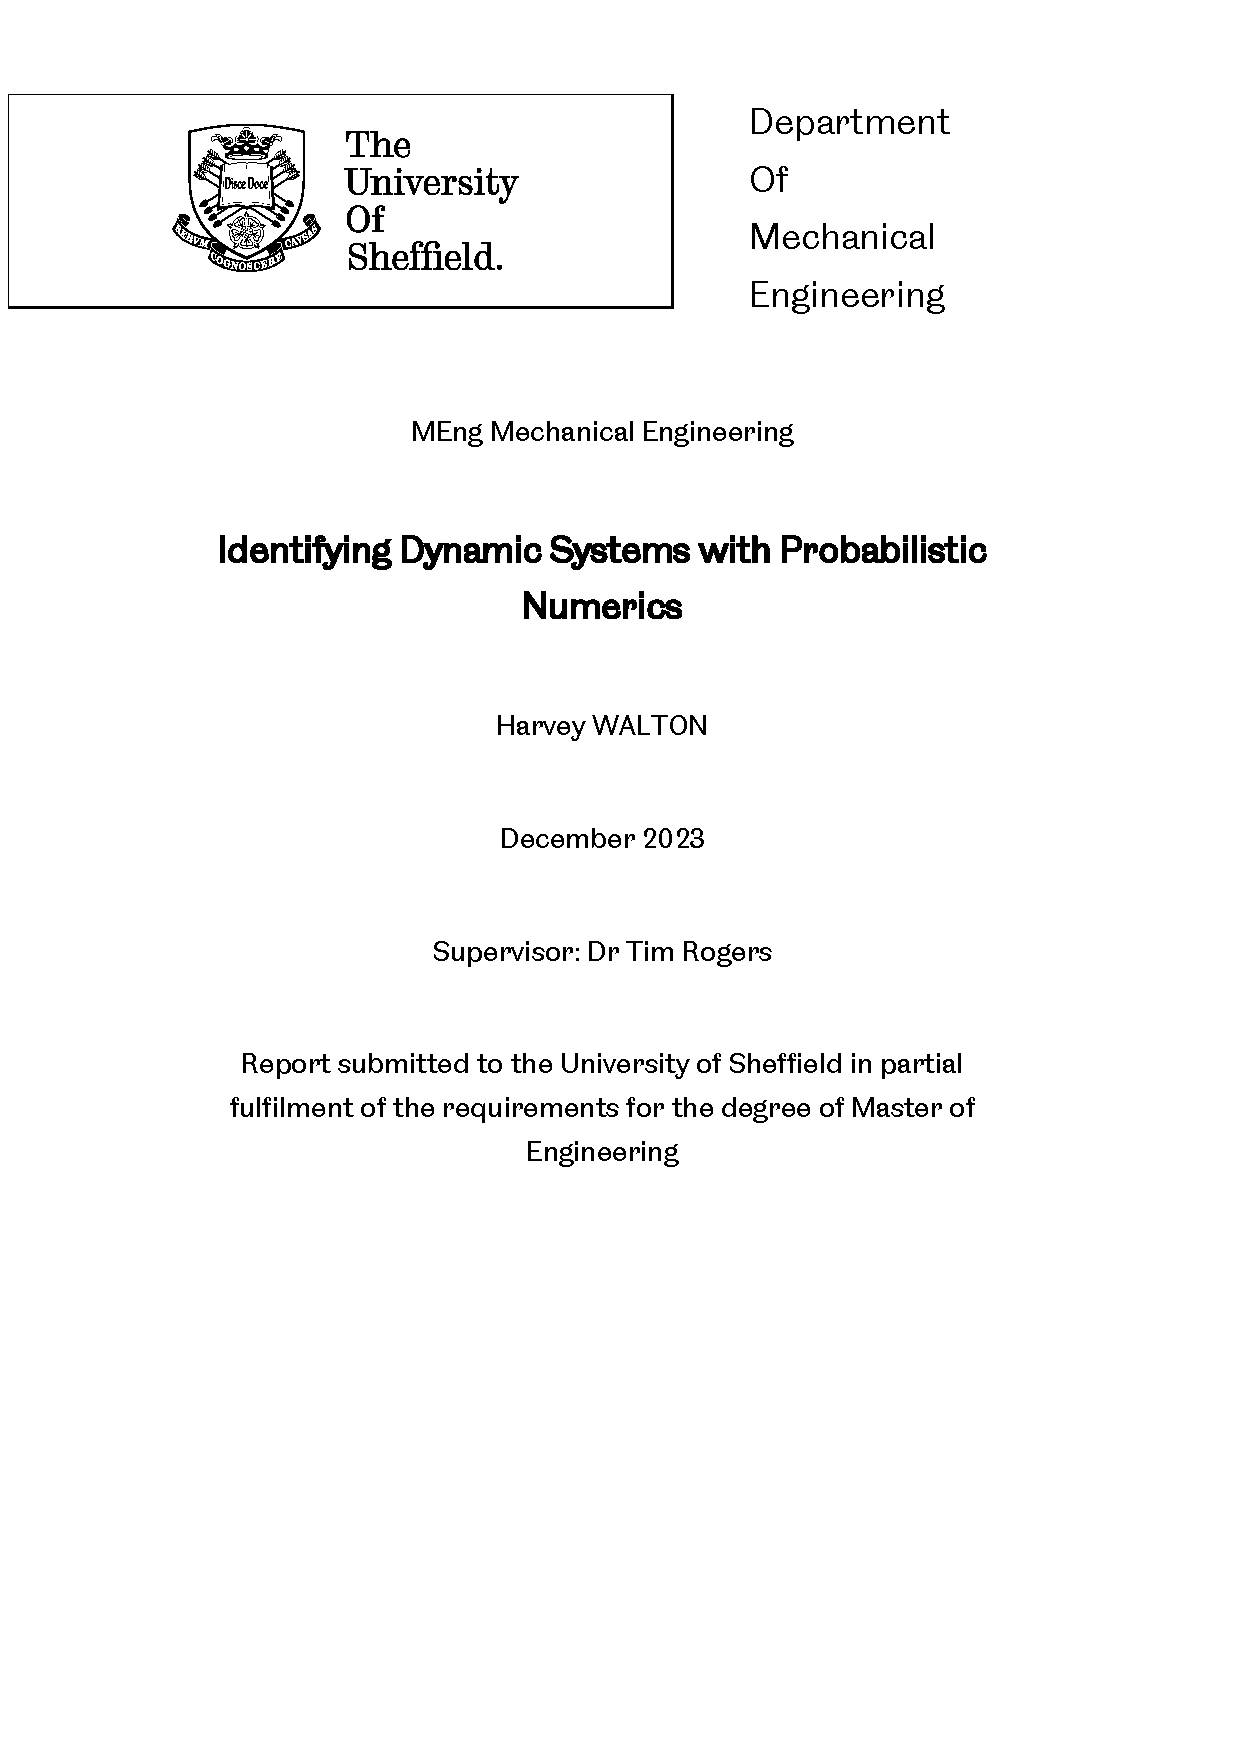
\includepdf[pages=1, frame, scale=1.09, pagecommand={}, offset=0 -35]{figures/titlepage.pdf}

    \printnomenclature

    \newpage
    \tableofcontents
    \newpage

    \pagenumbering{arabic}

    \section{Background and Understanding of the Problem}

    \subsection{Dynamic Systems}
    In mechanical engineering, the field of dynamics studies how systems, like structures and fluids, respond and evolve over time under varying forces.
    These forces can range from aerodynamic pressures to impacts from waves or road irregularities.
    Excessive vibration or oscillation of machinery is known to reduce service life and in extreme cases cause catastrophic failure.
    Therefore, by studying these dynamic systems they could be designed to perform better, be safer and to have lower maintenance costs.
    However, the field of dynamics is far from being mastered since there are many types of problems that cannot yet be solved.
    To begin with, here are some examples of dynamic systems:
    \begin{enumerate}[listparindent=\parindent]
        \item Firstly, a motorcycle suspension system is a combination of springs, dampers and linkages that connect the motorcycle chassis to its wheels.
        Its primary purpose is to keep the tyres in contact with the ground and without proper suspension, the tyres would lose traction when encountering bumps especially when braking, accelerating or cornering~\cite{UTI2020MotorcycleSuspension}.
        It is designed to allow some relative motion between the two in order to absorb impacts while at the same time trying to maintain its equilibrium position, and zero velocity (both relative to the chassis).

        The dampers in the suspension produce a force proportional to the velocity that acts to slow the wheel down.
        Viscous dampers do this by pushing a liquid though a small orifice as the wheel moves.
        Damping can be optimised (or made ``critical'') by bringing the system back to equilibrium after a disturbance as fast as possible.
        Too little damping, and the wheel will overshoot and oscillate back and forth before reaching equilibrium.
        Too much damping, and the wheel will not oscillate, but it will reach equilibrium more slowly than optimal.

        Similarly, the springs create stiffness in the system that produces a force with a magnitude proportional to the displacement of wheel which acts to return the wheel to its equilibrium position.
        Too high of a stiffness means that the system will not have enough time to absorb the impact softly, but too low means that the bike's responses to steering inputs are too slow and unreactive.

        Studying this dynamic system could allow for the prediction of behaviour based on varying these parameters.
        This would enable optimisation without trial and error, conserving resources during the research and development phase of the product lifecycle.

        \item Secondly, offshore wind turbines are known to experience high cycle fatigue (HCF) due to a relentless random forcing the waves that repeatedly crash against the base of its tower.
        This is a phenomenon that causes any micro-defects to grow into cracks over time due to cyclic loading below the elastic limit of the material, which reduces the life of the structure due to increased risk of mechanical failure.

        The rate at which this occurs increases with the amplitude of the stresses in the structure, which in turn increase with the amplitude of oscillation in response to this cyclic loading.
        If a periodic force is applied to any system with a specific frequency known as a resonant frequency, the amplitude of the oscillation may become very large even for a small amplitude force, leading to an excessive rate of high cycle fatigue.
        The same can happen in the case of the wind turbine that receives a random force with an \textit{average} frequency similar to this resonant frequency.
        It is even possible for the stresses in a structure to become so large that they exceed the ultimate tensile strength of the material, causing a sudden mechanical failure and the collapse of the turbine.

        Therefore, to make structures safer and reduce maintenance costs, it would be valuable to be able to model their dynamic properties such as this resonant frequency from system parameters such as the stiffness of the tower so that the frequencies at which they occur can be designed away from the expected frequencies of the periodic forces.

        \item Finally, an aircraft wing bends in response to aerodynamic forces.
        However, the forces themselves change as the wing twists and bends.
        The interdependence of these two effects creates complicated interactions that are difficult to model accurately.
        But it is important to do so because if at high airspeed, energy from the wing forcing is added to the system faster than it can be dissipated, the positive feedback loop can lead to a phenomenon called aerodynamic flutter where the oscillations become larger and larger until they cause catastrophic failure.
    \end{enumerate}

    \subsection{Identifying Dynamic Systems}

    So, dynamic systems have parameters such as mass, stiffness and damping coefficient which are fundamental characteristics of the system.
    ``Forwards modelling'' is when the observable behaviour of the system, known as the system properties, are predicted from the system parameters using physical laws.
    These properties include the resonant frequencies which are the forcing frequencies that produce a peak in amplitude of excitation, and the damping ratios which compare the damping coefficient to that of critical damping at each resonant frequency.

    Often a distinction is made between linear and nonlinear systems.
    Only linear systems comply with the principle of superposition, which states that ``when two or more waves simultaneously pass through a point, the disturbance at the point is given by the sum of the disturbances each wave would produce in absence of the other waves''~\cite{StudyComSuperposition}.
    This means that if you double the input force over time, the response over time is exactly double, but otherwise identical.
    This is not the case for nonlinear systems (such as the aircraft wing in the example above) where non-compliance with the principle of superposition causes the system properties to distort as the magnitude of the input force is increased.
    This, in turn, causes the response to become highly complex and chaotic, meaning that it is highly sensitive to initial conditions.
    This is why forward modelling is currently too difficult for systems that are non-linear.

    Unfortunately, everything is non-linear in real life.
    Only in rare cases are systems close enough to being linear that they can be approximated as such.
    What's worse is that even if a model did exist to solve the nonlinear system, it would be of no use because typically not even the system parameters are known to be able to input them into the model.
    This is why the field of dynamics has not been mastered, and all that can currently be done for medium to highly non-linear systems - \textit{which is almost all systems} - is to take real life data measurements from an existing system and identify the system properties and parameters that best fit the observed data through what is known as ``inverse modelling''.
    However, even this process is fraught with issues and uncertainty.

    \subsection{Classically Quantifying Uncertainty with Error Bounds}
    Identifying system properties and parameters using this inverse modelling approach results in values that are not exact, but have an uncertainty associated with them that comes from multiple sources.
    The first source of uncertainty is noise that is always present to some degree in sampled input data due to the measuring devices - typically accelerometers - that are used to capture the force input and corresponding response from the system.
    Furthermore, even if the true input and response could be sampled exactly, the non-identifiability problem states that since there are multiple sets of system parameters that could give the same set of observed outputs, it's impossible to uniquely determine them.
    Similarly, many algorithms make use of mathematical objects (such as matrix pseudoinverses) which have multiple alternatives - any of which could be used - where the correct choice is subjective.
    This noise and lack of uniqueness is reflected in the outputted system properties and parameters as uncertainty.


    Time passes continuously forever, and the governing equations of dynamic systems are defined mathematically in the continuous domain.
    In theory, these could be solved ``analytically'' to give an exact mathematical solution in the continuous domain.
    But in practice, data sampled from the real world is usually discrete, meaning that it is defined over a finite set of points separated by a finite time interval.
    In addition, many sets of governing of equations are currently too complex to solve analytically for systems that are not highly idealised.
    This is why when modelling, problems are classically solved using ``numerical methods'', which are discrete approximations of analytical solutions of the governing equations.
    Here, uncertainty of values is often quantified using error bounds derived from sensitivity analysis.
    For instance, the error bound of a stiffness could be represented as $0.1 \pm 0.02 Nm^{-1}$, indicating the expected range of the true value.
    This process involves estimating the uncertainty of input data, usually from the measuring equipment's resolution or variability in sample data.
    From these estimates, upper and lower bounds of the output parameters can be calculated.
    However, this is not straightforward and typically requires additional techniques and considerations beyond the core algorithm.


    \subsection{The Fourier Transform and the Frequency Response Function (FRF)}

    When inverse modelling during the analysis of dynamic systems, any collected time series data is almost always converted into the frequency domain, meaning the output becomes a function of frequency instead of a function of time.
    This is because it gives the physical meaning of the system properties a clear visual interpretation.
    Specifically, the Frequency Response Function (FRF) is computed, which is the ratio between the response and input in the frequency domain.
    This function is complex, which means it has two components that provide the amplitude (magnitude) and phase (lag) of the response vs the input.
    If the system parameters (mass, damping coefficient or stiffness) change, so do the system properties (resonant frequency and damping ratio).
    This is visible in the FRF in Figure~\ref{fig:frequency-response-function}, where a larger resonant frequency creates a peak in excitation at a higher frequency, and a lower damping ratio results in a sharper peak.
    Note the phase shifts by $\pi$ rad ($180\degree$) across a resonant frequency.

    \begin{figure}[ht]
        \centering
        \includegraphics[width=0.8\linewidth]{figures/frequency-response-function/frequency-response-function_}
        \caption{The magnitude and phase of $H(\omega)$, a frequency response function of a single-degree-of-freedom (SDOF) system for an acceleration measured in response to an input force, showing how changing its system parameters mass $m$ [$kg$], damping coefficient $c$ [$N \cdot s \cdot m^{-1}$] and stiffness $k$ [$N \cdot m^{-1}$] affects the system parameters resonant frequency $\omega_r$ [$rad \cdot s^{-1}$] and damping ratio $\zeta$ [$-$].}
        \label{fig:frequency-response-function}
    \end{figure}

    The decomposition of the input and response functions from the time domain to the frequency domain uses a linear transformation called the Fourier Transform, $F(\omega)$, as defined in Equation~\ref{eq:ft}

    \begin{equation}
        F(\omega) = \int_{-\infty}^{\infty} f(t) e^{-i \omega t} \, dt\label{eq:ft}
    \end{equation}
    \nomenclature[L05]{$F(\omega)$}{Fourier Transform of $f(t)$}
    \nomenclature[G08]{$\omega$}{Angular frequency}


    \noindent where $\omega$ is the angular frequency and $f(t)$ is the time domain latent function being transformed.
    This is an extremely powerful analytical technique that is used widely in engineering.
    However, for it to be applied in its base form to a function, this function must be defined for every point in time in the continuous domain $-\infty \text{ to } \infty$.
    Therefore, when working with sampled real world data, an approximation of this function is classically found using a numerical method called a Discrete Fourier Transform, specifically the Fast Fourier Transform (FFT).

    \subsection{The Fast Fourier Transform Algorithm}
    Although discovering this fast way to compute the Discrete Fourier Transform revolutionised many engineering disciplines such as structural health monitoring, image compression, signal processing, and control theory~\cite{Byjus2023}, its implementation has a number of challenges that have to be carefully handled.
    Firstly, the Fast Fourier Transform (FFT) assumes the input signal is periodic, which can lead to a phenomenon called spectral leakage if the signal is not an exact multiple of the chosen window~\cite{MathStackExchange2023}.\nomenclature[L04]{FFT}{Fast Fourier Transform}
    This can cause sharp resonance peaks to be smoothed out in the output because energy that should be concentrated at a peak frequency is spread across a range of frequencies nearby.
    But most importantly, the FFT can be highly sensitive to noise in the data, meaning a small amount of noise can create large fluctuations in the shape of the frequency spectrum, masking the true underlying frequencies and modal properties~\cite{MathStackExchange2023}.

    \subsection{Probabilistic Numerics and the Gaussian Process}
    This paper proposes a new method of performing the Fourier Transform and other linear transformations using a ``Gaussian Process'' (GP) that may be more robust to noise than the FFT through its use of probabilistic numerics.
    This is a new paradigm that seeks to expand on traditional numerical methods by incorporating probabilistic reasoning into the process of computation by treating ``a numerical problem as one of statistical inference instead''~\cite{ProbabilisticNumerics2023}.
    Here, uncertainty of outputs is modelled with a probability distribution as opposed to the error bounds as in traditional numerical methods.

    A GP uses noisy, discrete sampled data to model the probability distribution of a continuous ``latent'' function, $f(x)$, that represents the underlying relationship between an input, $x$, and an output, $f(x)$.\nomenclature[L06]{$f(x)$}{Latent function of the variable $x$}\nomenclature[L08]{GP}{Gaussian Process}
    In essence, it is ``a collection of random variables, any finite number of which have a joint Gaussian distribution''~\cite{rasmussen2006gaussian} which describes how the probability distribution of each variable depends on the other variables.
    These variables are outputs of the latent function at a specific input point and include both the training data (noisy observed samples at points in time), and the prediction points at which the true value is unknown.

    Assuming a mean of the latent function of zero, and a noisy observed force, $y_n = f(x_n)+\epsilon_n$, where $\epsilon_n \sim \mathcal{N}(0, \sigma^2_y)$, this joint distribution of the observed data and the latent, noise-free function at the test points is given~\cite{murphy2023probabilistic} by Equation~\ref{eq:joint-distribution}

    \begin{equation}
        \begin{pmatrix}
            \mathbf{y} \\
            \mathbf{f}_*
        \end{pmatrix}
        \sim \mathcal{N} \left(
        \begin{pmatrix}
            \boldsymbol{\mu}_X \\
            \boldsymbol{\mu}_*
        \end{pmatrix},
        \begin{pmatrix}
            \mathbf{K}_{X,X} + \sigma^2_y \mathbf{I} & \mathbf{K}_{X,*} \\
            \mathbf{K}_{X,*}^T & \mathbf{K}_{*,*}
        \end{pmatrix}
        \right)\label{eq:joint-distribution}
    \end{equation}

    \nomenclature[L22]{$y_n$}{Noisy observed output based on the latent function, $f(x)$}
    \nomenclature[L21]{$\mathbf{y}$}{A vector of $y_n$ values from a set of training points}
    \nomenclature[L07]{$\mathbf{f}_*$}{is a vector of function values at a set of test points $\mathbf{X}_*$}
    \nomenclature[L09]{$\mathbf{I}$}{Identity matrix}
    \nomenclature[L11]{$\mathbf{K}_{X,X}$}{Covariance matrix for training input data, $X$}
    \nomenclature[L12]{$\mathbf{K}_{X,*}$}{Covariance matrix between training inputs and test inputs, $\mathbf{X}$ and $\mathbf{X_*}$ respectively}
    \nomenclature[L13]{$\mathbf{K}_{*,*}$}{Covariance matrix for test inputs, $\mathbf{X}_*$}
    \nomenclature[G01]{$\epsilon_n$}{Noise in observation, normally distributed with a mean of zero and a variance of $\sigma^2_y$}
    \nomenclature[L23]{$\boldsymbol{X}$}{A vector of training point inputs}
    \nomenclature[L24]{$\boldsymbol{X}_*$}{A vector of test point inputs}
    \nomenclature[G07]{$\sigma^2_y$}{Variance of observation noise}
    \nomenclature[G03]{$\boldsymbol{\mu}_X, \boldsymbol{\mu}_*$}{Vectors containing the mean of the distribution of values of the latent function, at the training points, $\mathbf{X}$, and test points $\mathbf{X}_*$ respectively}
    \nomenclature[L10]{$\mathbf{K}_{\mathbf{A},\mathbf{B}}$}{Covariance matrix of the kernel function, $k(a,b)$, evaluated for each pair of elements a, b in vectors $\mathbf{A}$, $\mathbf{B}$}

    \noindent where $\epsilon_n$ is the observational noise; $\mathbf{y}$ is a vector of $y_n$ values from a set of training points; $\boldsymbol{\mu}_X$ and $\boldsymbol{\mu}_*$ are a vectors containing the mean of the distribution of values of the latent function, at the training and test points, $\mathbf{X}$ and  $\mathbf{X}_*$ respectively; $\mathbf{f}_*$ is a vector of function values at a set of test points $\mathbf{X}_*$; $\mathbf{I}$ is the identity matrix and $\mathbf{K}_{X,X}$, $\mathbf{K}_{X,*}$ \& $\mathbf{K}_{*,*}$ are a type of covariance matrix, $\mathbf{K}(\mathbf{A},\mathbf{B})$, based on the ``kernel'' function, $k(a,b)$ that is evaluated for each pair elements in the vectors $(\mathbf{X},\mathbf{X})$, $(\mathbf{X},\mathbf{X}_*)$ and $(\mathbf{X}_*,\mathbf{X}_*)$ respectively.
    Note that block matrix notation is used where matrices are conjoined to form a larger block matrix.

    The kernel is type of function that measures the similarity between each pair of inputs based on a set of hyperparameters and is chosen to reflect any prior knowledge about the problem domain.

    These hyperparameters need to be optimised by minimizing the Negative Log Marginal Likelihood (NLML), as defined~\cite{murphy2023probabilistic} in Equation~\ref{eq:NLML}\nomenclature[L19]{NLML}{Negative Log Marginal Likelihood}

    \begin{equation}
        -\log p(\mathbf{D}|\boldsymbol{\theta}) = \frac{1}{2} (\mathbf{y} - \boldsymbol{\mu}_X)^T \mathbf{K}_{\sigma}^{-1} (\mathbf{y} - \boldsymbol{\mu}_X) + \frac{1}{2} \log |\mathbf{K}_{\sigma}| + \frac{N}{2} \log(2\pi)\label{eq:NLML}
    \end{equation}

    \nomenclature[L03]{$\mathbf{D}$}{Training data}
    \nomenclature[G02]{$\boldsymbol{\theta}$}{Set of hyperparameters}
    \nomenclature[L14]{$\mathbf{K}_{\sigma}$}{Covariance matrix with noise term, $\mathbf{K}_{X,X} + \sigma^2_y \mathbf{I}$}
    \nomenclature[L18]{$N$}{Number of training points}

    \noindent where $\mathbf{D}$ is the training data; $N$ is the number of training points; $\boldsymbol{\theta}$ is the set of hyperparameters and $\mathbf{K}_{\sigma} = \mathbf{K}_{X,X} + \sigma^2_y \mathbf{I}$ is the covariance matrix with the noise term.
    This measures how well the model explains the observed data for a given set of hyperparameters while penalizing complexity to avoid overfitting, which is when the model fits the training data so well that it generalises poorly to new test data.
    This can happen when the model has not only learnt the underlying function but also its associated noise, which will not be consistent between datasets due to its random nature.
    Optimisation in this manor works by identifying the hyperparameter values that are most likely to produce the observed training data.

    To predict the latent function at one or multiple points, the ``posterior'' probability distribution of the function is determined by updating the initial prior assumptions its shape using the training data.
    This process is called conditioning the joint Gaussian prior distribution on the observations~\cite{rasmussen2006gaussian}, as shown in Equation~\ref{eq:18.51}, where $\boldsymbol{\mu}_{*\vert \mathbf{X}}$ and $\boldsymbol{\Sigma}_{*\vert \mathbf{X}}$ are the conditional mean and covariance of the GP, given the training data, $\mathbf{X}$ as shown in Equation~\ref{eq:18.52} and Equation~\ref{eq:18.53} respectively.

    \begin{equation}
        p(\mathbf{f}^* \vert \mathbf{D}, \mathbf{X}^*) = \mathcal{N}(\mathbf{f}^* \vert \boldsymbol{\mu}_{*\vert \mathbf{X}}, \boldsymbol{\Sigma}_{*\vert \mathbf{X}})\label{eq:18.51}
    \end{equation}

    \begin{equation}
        \boldsymbol{\mu}_{*\vert \mathbf{X}} = \boldsymbol{\mu}_* + \mathbf{K}_{X,*}^T (\mathbf{K}_{X,X} + \sigma^2_y \mathbf{I})^{-1} (\mathbf{y} - \boldsymbol{\mu}_X)\label{eq:18.52}
    \end{equation}

    \begin{equation}
        \boldsymbol{\Sigma}_{*\vert \mathbf{X}} = \mathbf{K}_{*,*} - \mathbf{K}_{X,*}^T (\mathbf{K}_{X,X} + \sigma^2_y \mathbf{I})^{-1} \mathbf{K}_{X,*}\label{eq:18.53}
    \end{equation}

    \nomenclature[G04]{$\boldsymbol{\mu}_{*\vert \mathbf{X}}$}{Conditional mean of the Gaussian Process, given the training data, $\mathbf{X}$}
    \nomenclature[G05]{$\boldsymbol{\Sigma}_{*\vert \mathbf{X}}$}{Conditional covariance of the Gaussian Process, given the training data, $\mathbf{X}$}

    Note that this GP is closed under the action of linear operators which means that it can be described using only a combination of operations that comply with the principle of superposition.
    It is also defined in the continuous domain $-\infty \text{ to } \infty$ so the Fourier Transform can be taken analytically without needing to resort to the discrete FFT\@.
    Incredibly, since the Fourier Transform is also a linear transformation, the result of this transformation of the GP is yet another GP\@.
    Therefore, modelling this way provides an inherent mechanism to account for uncertainty and allows this information to be preserved naturally when performing transformations of the data.
    Furthermore, the noise term  $\epsilon_n \sim \mathcal{N}(0, \sigma^2_y)$ explicitly models the observational noise, giving the GP a way to distinguish between the signal and noise components.
    This is why the use of probabilistic numerics may allow for Fourier Transform to be performed with better robustness to noise.

    \subsection{Implications of the Findings}

    \subsubsection{Implications in the Context of the Fourier Transform}

    A Fourier Transform method that can be applied to discrete data and is more robust to noise than the FFT would have significant implications in various fields of engineering.

    In the context of dynamic systems, the system properties and parameters could be identified more precisely.
    This is especially true for nonlinear systems whose complex dynamic behaviours can be obscured by noise such as two closely spaced resonant frequencies that may be mistaken for a single one.
    Consequently, this would allow earlier detection of changes in structural integrity in the context of Structural Health Monitoring because an increase in nonlinear behaviour is typical of the formation or growth of cracks or other defects.
    Therefore, engineers would be able to make and maintain structures with greater safety by increasing the likelihood of detecting structural damage before catastrophic failure occurs.

    A Fourier Transform that is more robust to noise could improve other areas of engineering where it is used extensively such as control theory, signal processing, image processing, and acoustic engineering.
    In these contexts, it is used to simplify a computationally expensive operation in the time domain called a convolution into a simple pointwise multiplication in the frequency domain.
    Therefore, this improvement would enhance operations like signal filtering, image edge detection and acoustic noise reduction by reducing the distortion that occurs during these operations due to the presence of noise in the input data.

    More generally, this alternative method of modelling uncertainty using probabilistic numerics via a Gaussian Process (GP) could be employed to improve robustness to noise where classically, other numerical methods would need to be implemented to linearly transform discrete data.

    \section{Aims and Objectives}
    \subsection{Aim}
    The main aim of this paper is to improve the noise resilience of time series data when converted to frequency domain.

    \subsection{Objectives}
    This overarching aim can be broken down into four objectives, plus an optional stretch objective if time allows:
        \begin{enumerate}
            \item Get a working Gaussian Process model, which involves:
                \begin{itemize}
                    \item Choosing and creating a kernel.
                    \item Implementing optimisation of kernel hyperparameters. \label{item:nll}
                    \item Creating a prediction function to predict the outputs of new inputs. \label{item:predict}
                \end{itemize}
            \item Scale to large data by implementing a Sparse GP approximation.
            \item Adjust this model to enable the closed form Fourier Transform to be found.
            \item Compare the noise resilience with existing Discrete Fourier Transform methods such as the Fast Fourier Transform.\label{noise-resilience}
            \item Stretch Objective: Compare the smoothing out of sharp resonance peaks due to spectral leakage.\label{stretch-obj}
        \end{enumerate}

    \section{Work Completed to Date}
    The first thing needed to be complete was the basic Gaussian Process model.
    This was implemented using the programming language Python and consisted of the following components:
    \subsection{The Data}
    Previously collected turbine tap test data~\cite{MEC326} was converted to a .csv file (a file that formats data into table of values), and imported into python.
    The test data consisted of accelerometer data from the tip of a hammer as well as a single location on a turbine blade when struck at 10 positions.
    This was sampled at a rate of $16,384 Hz$ for just under 4 seconds.
    For simplicity, only the response data at the first position was imported, and initially a small set of 100 samples was selected from the centre (to reduce computation time).
    This time series acceleration data, as shown in the ``Force Response Over Time'' plot in Figure~\ref{fig:input-response-plot}, was used as training data to be fit by the GP\@.

    \begin{figure}[ht]
        \centering
        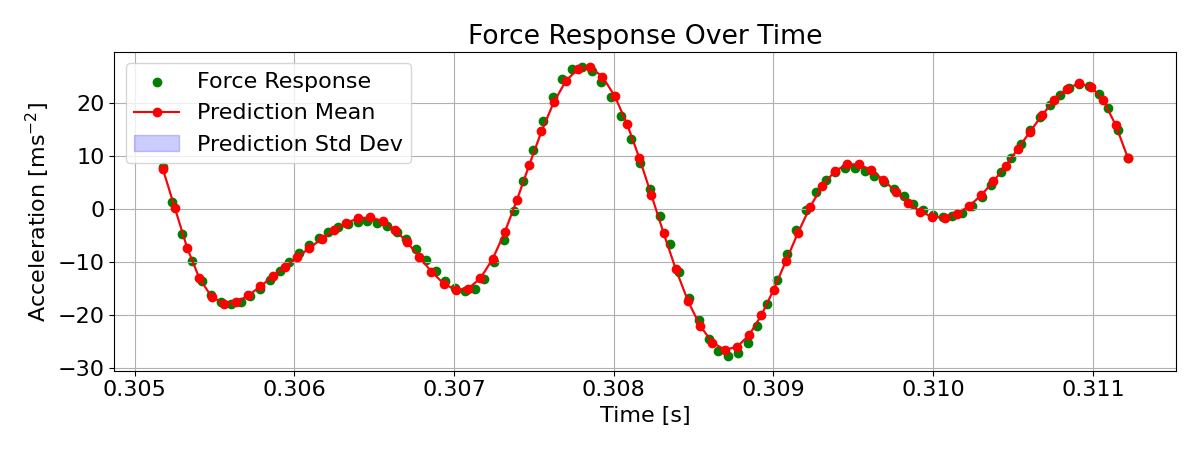
\includegraphics[width=1.0\linewidth]{figures/input-response-plot/input-response-plot.png}
        \caption{The time series training data, and the mean and standard deviation of the GPs prediction of its latent function. Note that the prediction functions are continuous but must be evaluated at a discrete set of points in order to be plotted.}
        \label{fig:input-response-plot}
    \end{figure}



    \subsection{The Kernel}
    A Squared Exponential Kernel~\cite{duvenaud2014kernel} was chosen to reflect the nature of the sample data that is continuous and smooth, with no sudden jumps.
    In addition, it only has two hyperparameters, and this low number speeds up their optimisation process compared to alternative kernels.
    This function is defined in Equation~\ref{eq:se-kernel}

    \begin{equation}
        k(a,b) = \sigma^2 \exp\left(-\frac{(a - b)^2}{2l^2}\right) \label{eq:se-kernel}
    \end{equation}
    \nomenclature[L15]{$k(a,b)$}{Kernel function, evaluating the similarity of points $a$ and $b$}
    \nomenclature[L02]{$a, b$}{Elements of vectors $\mathbf{A}, \mathbf{B}$ respectively}
    \nomenclature[L01]{$\mathbf{A}, \mathbf{B}$}{Vectors with elements $a, b$ - subcript indicates index of element}
    \nomenclature[G06]{$\sigma^2$}{The variance hyperparameter of the SE kernel}
    \nomenclature[L16]{$l$}{Length scale hyperparameter of the SE kernel}

    \noindent where $k(a,b)$ is the kernel function evaluated at elements $a_i$, $b_j$ of vectors $\mathbf{A}$, $\mathbf{B}$ respectively; $\sigma^2$ is the variance hyperparameter and $l$ is the length scale parameter.

    The variance hyperparameter, $\sigma^2$, determines the average distance of the function away from its mean.
    It is a simple scale factor present in all kernels.
    Finally, length hyperparameter, $l$, determines how smooth or wiggly the function is, i.e., how fast the function can change direction.

    \subsection{Hyperparameter Optimisation}
    An algorithm was designed to optimise the hyperparameters of the kernel by minimising the Negative Log Marginal Likelihood (NLML), for which a method was written (Appendix.~\ref{app:GPT}).
    It did this by modifying each hyperparameter randomly in turn and seeing if the NLML improved.
    This was repeated for up to 100 iterations.

    Imagine if the hyperparameter was only updated the new NLML was lower than the previous.
    Since the shape of a cost function can be complex and highly dimensional, the algorithm could have got stuck in what is known as a local minimum and never find the global minimum.
    This would be analogous to a ball that ``tried'' to find the bottom of a valley by rolling directly downhill.
    If it got stuck in a small ditch half-way down the larger hill, it would never find the lowest point.

    Therefore, a mechanism was added to the algorithm to avoid this:
    If the new NLML was higher (i.e., worse) than the previous, the hyperparameter was maybe still updated, with a larger probability the closer the NLML was to the previous NLML\@.
    When the last iteration was complete, the lowest NLML of all the combinations hyperparameters was selected.
    This allowed the algorithm to explore after reaching a minimum to potentially find another part of the NLML function that was lower.

    \subsection{Predict Function}
    The predict function was constructed, which accurately calculated the mean and standard deviation of the latent function as shown by the ``Prediction Mean'' and ``Prediction Std Dev'' plots in Figure~\ref{fig:input-response-plot}.
    Furthermore, when Gaussian noise was added to the input data, the standard deviation of the prediction became larger to take account for this noise, as shown in Figure~\ref{fig:input-response-noise}.


    \begin{figure}[ht]
        \centering
        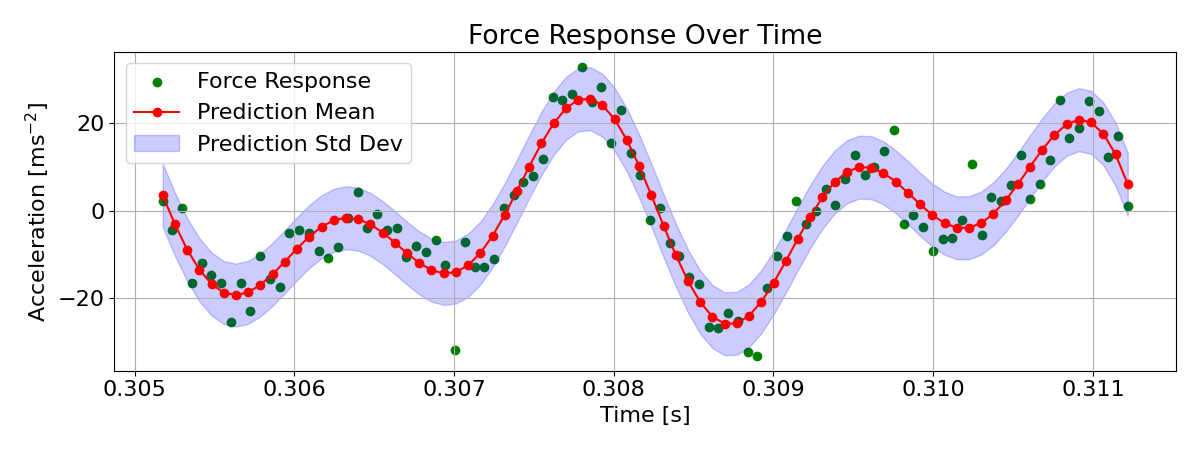
\includegraphics[width=1.0\linewidth]{figures/input-response-noise/input-response-noise.png}
        \caption{The prediction functions of the GP when noise was added to the training data, showing that the standard deviation of the prediction increased compared to Figure~\ref{fig:input-response-plot}.}
        \label{fig:input-response-noise}
    \end{figure}

    \section{Plan for Future Work}
    Firstly, the Sparse GP approximation known as the Fully Independent Training Conditional (FITC) will be complete to allow the model to scale to large data~\cite{q-candela}.
    This will reduce the complexity of the training phase from $O(N^3)$ to $O(MN^2)$, where M is a set of inducing points chosen to be a subset of the original training points, evenly spaced, and $N \gg M$. \nomenclature[L17]{$M$}{Number of inducing points in Sparse GP} \nomenclature[L20]{$O()$}{Big O notation, used to describe the complexity - or ``order'' of an algorithm}
    This modification will be made to both the NLML and predict functions, which requires a very specific implementation in order to keep the calculations numerically stable and efficient in terms of computation time and memory required.

    After this is complete, the hyperparameters can be optimised and the GP can be fit for functions containing more than 10,000 data points in a significantly reduced computation time.

    Next, the input space of the joint Gaussian distribution will be extended to the frequency domain by incorporating the Fourier Transform.

    Then, a method to compare the robustness to noise of the Fourier transform computed using the GP model vs the classical FFT model needs to be determined (Objective~\ref{noise-resilience}).
    One method of doing this uses the (discrete) Mean Squared Error (MSE), which is an algorithm used to measure the quality of an estimator (lower is better) using the average of the squares of the differences between the points at each index position in the series, as shown in Equation~\ref{eq:mse}

    \begin{equation}
        \text{MSE} = \frac{1}{n} \sum_{i=1}^{n} (a_i - b_i)^2
        \label{eq:mse}
    \end{equation}

    \noindent where $a_i$, $b_i$ are the values of vectors $\mathbf{A}$, $\mathbf{B}$ at index i.
    The method works as follows:

    First, the Fourier Transform of the data can be computed using each method.
    Then, some Gaussian noise can be added to the data and the Fourier Transform can be computed again using both methods.
    Next, for the standard FFT method, the Mean Squared Error can be computed between Fourier Transforms of the unmodified and noisy data.
    Similarly, for the Gaussian Process method, the MSE can be computed between the mean functions of Fourier Transforms of the unmodified and noisy data.
    Since these mean functions are continuous, to compute the MSE they first need to be discretised by evaluating them at the same frequencies present in the FFTs generated using the first method.
    The two MSEs can then be used to make a comparison between robustness to noise of each method.
    This could be repeated for different levels and types of noise (Gaussian vs white noise) to test how each method performs under various conditions.

    If time allows the stretch objective (\ref{stretch-obj}) of comparing how smoothed out sharp resonance peaks are due to spectral leakage can be complete.
    To do this, the Fourier Transform of a pure sine wave should be found using both the GP and FFT methods.
    This is because it can be solved exactly on paper to provide a Fourier Transform with a sharp peak at the frequency of the wave.
    Each method can then be compared to the exact solution using the MSE to see which has peaks that are more distorted by spectral leakage.

    Finally, a conclusion can be drawn regarding the utility of the new Gaussian Process (GP) method of computing the Fourier Transform when compared to the classical Fast Fourier Transform (FFT) with respect to robustness to noise and prevention of artifacts due to spectral leakage in the context of dynamic systems.
    Since the addition of noise is an inherently random, the comparison should be repeated several times, and the conclusion should be drawn using a statistical technique called hypothesis testing.
    This provides a framework to state whether there is sufficient evidence to reject the default ``null'' hypothesis - that the new GP method is no better than classical methods in these respects - allowing a strong conclusion to be drawn regarding the improvements in noise resilience of time series data when converted to frequency domain through the implementation of probabilistic numerics.

   % \subsection{Future Work Time Plan}
    A Gantt chart outlining these main steps and the approximate schedule for the remaining work in the project is included (Figure~\ref{fig:gantt-chart_}).

    \begin{landscape}
        \begin{figure}[p] % 'p' places the figure on a page of its own
            \centering
            \includegraphics[width=\linewidth]{figures/gantt_chart/gantt-chart_.png}
            \caption{A Gantt chart showing work remaining, using a format modified from~\cite{DataCampGanttChart2021}. This includes scheduled delays in the Christmas and Easter holidays to allow for exam revision and as a buffer to catch up to the schedule if the project is falling behind.}
            \label{fig:gantt-chart_}
        \end{figure}
    \end{landscape}

    \FloatBarrier





    \newpage
    \printbibliography
    \addcontentsline{toc}{section}{References}
    \newpage
    \appendix
\section{The use of generative AI (ChatGPT)}
OpenAI's ChatGPT interface, powered by the GPT-4 large language model, was used to implement the Negative Log Marginal Likelihood (NLML) method in my code in a specific way to ensure numerical stability though the use of the ``Cholesky decomposition''.
The prompt and output is provided in Figure~\ref{fig:chat-NLML}.
\begin{figure}[htbp]
    \centering
    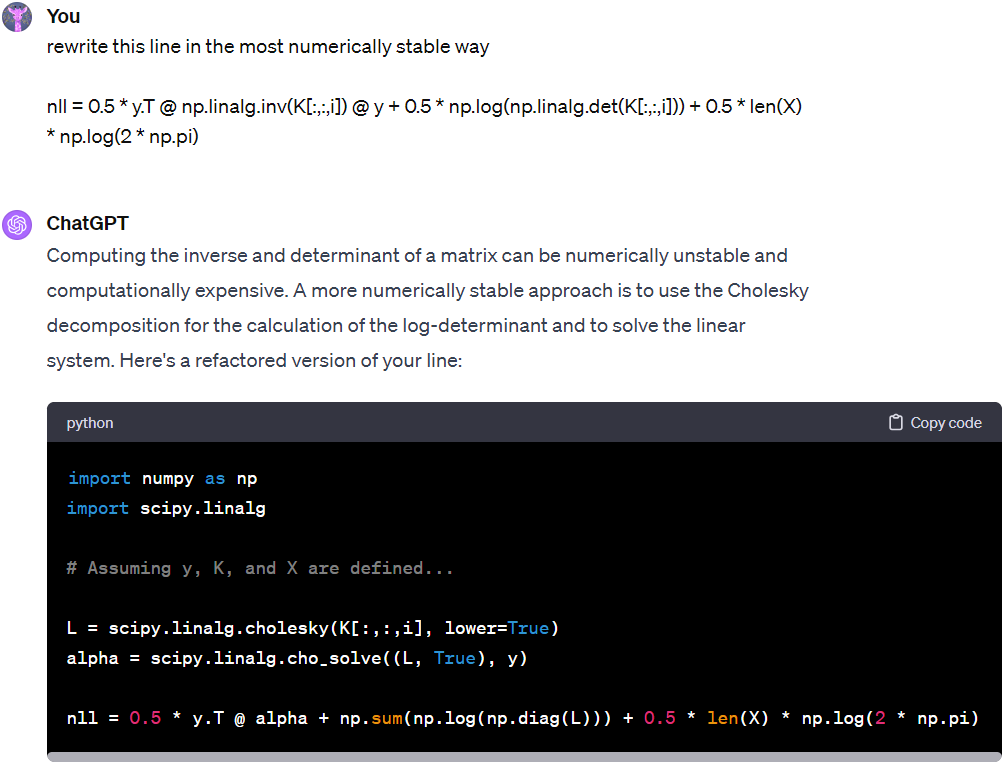
\includegraphics[width=1\linewidth]{figures/chat-NLML/chat-NLML.png}
    \caption{ChatGPT prompt and output providing a way to compute the NLML that is faster and more numerically stable}
    \label{fig:chat-NLML}
\end{figure}

\FloatBarrier

In order to ensure that this function was valid, its implementation was confirmed by the relevant literature~\cite{murphy2023probabilistic}~(Section 18.3.6).
After which, this function was simplified and adapted into that it could be to be added to the $gp\_model$ class as a method, and so that it would work with the way the input data was formatted, as shown in Listing~\ref{1st:NLML}

\begin{lstlisting}[caption={Method used to calculate the Negative Log Marginal Likelihood (NLML).} language=Python,label={lst:NLML}]
    def compute_nlml(self, hyperparameters):
    self.update_hyperparameters_and_debug(hyperparameters)
    self.reshape_X_and_y()

    if self.gp_algo == 'cholesky':
        K = self.gp_kernel.compute_kernel(self.X, self.X)
        K += np.repeat(np.array(np.eye(len(self.X)) * 1e-3)[:,:, np.newaxis], self.X.shape[1], axis=2)
        debug_K = np.squeeze(K)
        L = scipy.linalg.cholesky(K[:, :, 0], lower=True)
        n = len(self.y)
        one_vector = np.ones(n)
        y_adj = self.y - self.y_mean

        alpha = scipy.linalg.cho_solve((L, True), y_adj)

        term_1_c = (0.5 * y_adj.T @ alpha).item()
        term_2_c = np.sum(np.log(np.diag(L)))
        term_3_c = 0.5 * n * np.log(2 * np.pi)

        nlml = term_1_c + term_2_c + term_3_c

        out_c = {
            'nlml': nlml,
            'term_1': term_1_c,
            'term_2': term_2_c,
            'term_3': term_3_c
        }

        return out_c

\end{lstlisting}




\end{document}